\documentclass[11pt]{article}
\usepackage[utf8]{inputenc}
\usepackage[T1]{fontenc}
\usepackage{amsmath}
\usepackage{amsfonts}
\usepackage{amssymb}
\usepackage[version=4]{mhchem}
\usepackage{stmaryrd}
\usepackage{graphicx}
\usepackage[export]{adjustbox}
\graphicspath{ {./images/} }

\begin{document}
Private Equity Funds of Funds Investment Process

\section*{PE Funds of Funds Have Varying Investment Objectives}
There are many commonalities among PE FoFs. They offer investors diversified access to private equity, they aim to value-add by selecting top quartile PE funds, and they may potentially offer investors economics of scale and allocations to oversubscribed PE funds. However, not all PE funds of funds are the same. They differ by three key dimensions:

\begin{itemize}
  \item Geographical focus: Like direct PE fund investments, PE FoFs could focus on country, regional, or global portfolio companies. The preferred option typically depends on the size of the market opportunity. In the United States, it is common to see US-focused PE FoFs, while in Europe and Asia, PE FoFs tend to be regionally focused. This geographical focus allows PE FoFs to focus on the GP landscape. For example, it is estimated that there are over 800 different active GPs in Asia, which makes it challenging to pick the top performers. In addition, PE FoFs often seek to identify emerging PE funds to invest in before they become highly sought after. This often requires strong domain knowledge, local presence, and sufficient scale to be treated by PE funds as a preferred investor. There are also PE FoFs with a global focus. These tend to be fewer, and are normally part of a larger organization with a global footprint to provide the right market expertise and access to the best GPs.
  \item Focus: PE FoFs could focus on different types of GP categories such as venture capital, growth equity, or buyouts. Within buyouts there are also subcategories such as small, medium, large, and mega buyouts, depending on the deal size. PE FoFs may focus on a specific category and subcategories, or diversify across categories.
  \item Portfolio construction: When constructing a portfolio of PE funds, diversification can be achieved in several dimensions, including different strategies, GP, vintage year, industry, and geography. A right balance of diversification can reduce risk and enhance returns. Diller and Herger (2009) concentrated on two dimensions - the number of fund commitments per year and the number of vintage years - and found that diversifying across 15 funds over 3 to 5 vintage years can effectively reduce the loss of invested capital to zero and increase the average performance of a PE fund portfolio. In a similar study, Dompé (2019) used a different dataset and concluded that 20 to 25 PE funds is the optimal size for a portfolio of PE funds that is diversified across stages, vintages, and geographies. They also added that once an optimal point is reached, adding more funds has a negligible impact on risk reduction and could reduce the value added from manager selection.
\end{itemize}

\section*{Distinguish between Primary and Secondary PE Fund of Funds}
PE FoFs can be broadly categorized into the following strategies:

Primary Funds of Funds (primary FoFs) invest in individual PE funds at their inception through primary capital commitments. Depending on its strategy, a typical primary FoF may develop a portfolio of between 20 to 50 PE fund investments over several vintage years. Primary FoFs provide their investors with exposure to a diversified portfolio of PE funds and tend to demonstrate a similar J-Curve to that of an individual PE fund. As a mature category of the PE asset class, many primary FoFs employ specific strategies and focus on investing in PE funds of a specific region, strategy or fund size.

Secondary Fund of Funds (secondary FoFs) invest in individual PE funds by acquiring LP interests through a secondary market purchase. Session 4.2, Private Equity Funds, describes the concept of PE secondary market transactions. Depending on its strategy, a typical secondary FoF may develop a portfolio of several hundred LP interests and is generally significantly more diversified than primary FoFs. Secondary FoFs provide investors with exposure to a seasoned and diversified portfolio of PE funds and tend to demonstrate a shorter J-Curve than an individual PE fund. Given that many of the purchased funds have progressed beyond their initial vintage year, LPs may have visibility into the portfolio companies held in the underlying funds.

\section*{Describe the Process for Constructing a Portfolio of PE Funds}
The exhibit Typical Selection Process for PE Funds shows a typical process of constructing a portfolio of PE funds. It can be described in three phases.

Portfolio construction phase. An investor must first decide how many PE funds provide adequate diversification. As mentioned in earlier sections, the typical number of PE funds for a PE FoFs is between 15 and 50. Next, the investor must ensure consistent investment through the cycle. This means spreading the investment across vintage years. The total number of PE funds and the spread across vintage years will help the investor decide on the suitable size of their annual commitment. After deciding on the amount to commit, the investor can use top-down criteria to structure the portfolio. For example, the investor may want to consider geographical exposure, such as a target of $60 \%$ US, $20 \%$ Europe, $10 \%$ Asia, and $10 \%$ rest of world. The investor may also consider diversification across the categories, such as a target of $65 \%$ buyout, $10 \%$ growth, and $25 \%$ venture capital. If the investor decides to make 10 commitments each year, they can broadly determine how many funds in each category they will commit to each year.

GP and fund selection phase. The next phase is screening the GPs or the funds. Most investors would adopt a mix of quantitative and qualitative screens base on their portfolio construction parameters that broadly includes categories and geography. Investors may also include specific parameters based on their preference or risk management. An example is whether the GP has previously managed a successful fund. Some larger institutional investors typically avoid first-time funds because of their lack of track record. Another example is fund size. Investors generally do not want to take an overly disproportional size of the fund, so the fund size must match their target commitment size. Investors also make a qualitative assessment of the GPs' reputation, strategy, team, track record, network, and risk management. While an investor could screen for GPs, looking for the top-quartile GPs based on their historical performance, these GPs may not be fundraising. The fundraising cycle for GPs is typically one fund every two to three years for small GPs, and one fund a year for large GPs with multiple funds strategy. Nonetheless, the investor could still be introduced to the manager and aim to get on the GP's pre-marketing list when they are next fundraising. Alternatively, an investor may form a macro view and identify attractive areas for investment. They would then screen for funds that meet that investment strategy, geography, or niche. It is also important for investors not to rely solely on past performance due to the trend of declining performance persistence. Investors should also consider including emerging managers as part of their selection process.

Ongoing monitoring phase. After the closing of investment into PE funds, some of the key activities for the investor include:

\begin{itemize}
  \item Regular interaction with the GP to understand the status of underlying portfolio companies and the GP's outlook on risks and opportunities
  \item Regular performance analysis of the fund
  \item Regular valuation update of the fund
\end{itemize}

In addition, some investors may sit on the LP advisory board to monitor potential conflict of interest between the fund and GP. Most LP would attend annual LP meeting to get the update on the PE fund. The information from these activities may help the investor to refine their portfolio construction as market condition changes.

An investor choosing the PE FoF option will rely on the manager of the PE FoF to perform the portfolio construction required to build a diversified portfolio. Investors should evaluate the manager of the PE FoFs manager to determine whether the manager is able to select and access top quartile GPs for their fund.

\begin{center}
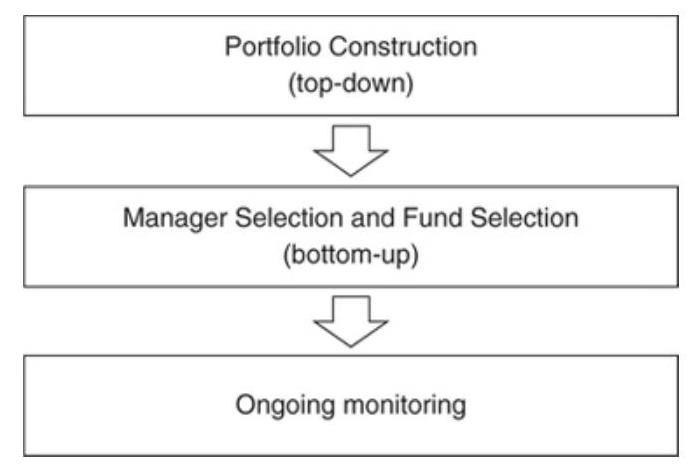
\includegraphics[max width=\textwidth]{2024_04_10_45ef17878a276b09aeb7g-3}
\end{center}

Typical Selection Process for PE Funds

Source: CAIA Association


\end{document}